\chapter{Teor\'ia y Fundamentos}

\def\baselinestretch{1.0}


%%% ----------------------------------------------------------------------
\medskip
Para dos o m\'as secuencias temporales, un aspecto importante a
considerar, nace de la siguiente pregunta �C\'omo resumir esta
informaci\'on de manera simple y compacta? Para esto es necesario
tener medidas o \'indices que resuman toda esta informaci\'on en
un s\'olo n\'umero.

 Dependiendo de la perspectiva que se plantee, en la literatura se puede encontrar muchas formas, por ejemplo la distancia Euclidiana. Por otra parte, Warren Liao (2005), hace una rese\~na de varias medidas de
asociaci\'on y medidas de similaridad para secuencias temporales y
algoritmos, para aplicar en el an\'alisis de Cluster.

Por otra parte, Chouakria y Nagabhushan (2007) proponen un
\'indice de disimilaridad adaptativo para medidas de proximidad en
series temporales, la cual se llama \textit{automatic adaptive
tuning function}. Rukhin y Vallejos (2008) introducen un
coeficiente de similaridad para secuencias Espaciales y
Temporales, donde este coeficiente, es una normalizaci\'on de una suma
de incrementos para secuencias de tiempo o espacio.

 En este Cap\'itulo revisaremos algunas medidas m\'as usadas de
asociaci\'on y similaridad. Tambi\'en, se ver\'an algunas definiciones
b\'asicas de procesos estoc\'asticos, con algunas hip\'otesis que
sustentan este Proyecto de Titulaci\'on, como es la estacionalidad
de las series temporales. Planteando tambi\'en la l\'ogica del
Coeficiente de Codispersi\'on y su interpretaci\'on.

\section{Definici\'on de Procesos Estoc\'asticos}

El Coeficiente de Codispersi\'on o de Comovimiento tiene la capacidad de captar el comportamiento respecto a si dos series se mueven juntas en el tiempo, en varias ocasiones esto se puede modelar a trav\'es de modelos param\'etricos que est\'an asociados a esta medida de Codispersi\'on. Primero es necesario definir algunos objetivos y estructuras que nos ayudar\'an a describir diferentes escenarios. Comenzaremos por la definici\'on de Procesos Estoc\'asticos.

\begin{defn}
Sea $X_{t}$  una funci\'on, \\
$$
\begin{array}{rccl}
X:&\Omega \times T &\longrightarrow&\mathbb R\\
&(\omega, t)&\mapsto&X(\omega,t)
\end{array}
$$\\
tal que para cada $t$ $\in$ $T$, $X_{t}(\omega)$ es una variable aleatoria. Llamamos al conjuno $\{X_t,t \in T\}$ Proceso Estoc\'astico sobre el espacio $\Omega$.
\end{defn}

Una secuencia $\{X_t, t \in T\}$ es fuertemente o estrictamente
estacionaria si $\{X_{t_1},\ldots,X_{t_{n}}\}$= $\{X_{t_1+h},\ldots,X_{t_{n}+h}\}$ en
distribuci\'on, para toda colecci\'on $t_1,...,t_n$ y para todo $h$ $\in$ $T$. Es decir, el proceso es invariante bajo traslaci\'on.

Por otra parte, una secuencia es d\'ebilmente, o de segundo orden
estacionario si:
\begin{enumerate}
  \item $\mathbb E(X_{t})=\mu $.
  \item $\mathbb V(X_{t})=\sigma^{2} $.
  \item $\mathbb Cov(X_{t},X_{t+k})=\gamma_{k}$. La funci\'on de autocovarianza es una funci\'on que depende \'unicamente de la distancia entre $t$ y $t+k$.
\end{enumerate}
%Entonces la secuencia $\{\gamma_k, k \in T\}$ es llamada funci\'on de autocovarianza.\\
Seguidamente se define:\\
         $\rho_{k}=\gamma_k\diagup\gamma_0$ y $\{\rho_k, k \in T\}$
es llamada funci\'on de autocorrelaci\'on (ACF) del proceso $\{X_{t}, t \in T\}$.\\
\\
Como caso particular cuando $T=\mathbb Z$, se est\'a en presencia de una serie temporal.

Entonces las series de tiempo son una realizaci\'on de los procesos estoc\'asticos. Ahora, en esta secci\'on se dar\'an algunas definiciones de modelos y/o procesos autoregresivos, de media m\'ovil y procesos ARMA.

\section{Ruido blanco}
%\begin{defn}
La secuencia ${\epsilon_{t}}$, consiste en variables aleatorias
independientes con media 0 y varianza $\sigma^{2}$. $\epsilon_{t}$ es llamada
ruido blanco. Esta serie es estacionaria de segundo orden con
$\gamma_{0}$=$\sigma^{2}$ y $\gamma_{k}$=0 ,$k \neq 0$.
%\end{defn}

\section{Procesos Autoregresivos}

Sea $\{X_{t},t \in Z\}$ un Proceso Estoc\'astico. Se dice que $\{X_{t}\}$ es un modelo autoregresivo de orden $p$ denotado
por AR($p$),si puede ser escrito por la ecuaci\'on:
\begin{eqnarray}
X_{t}&=&\sum_{r=1}^{p} \phi_{r}X_{t-r}+\epsilon_{t}, t \in T
\end{eqnarray}
donde $\phi_{r}$ son los par\'ametros del modelo y $\epsilon_{t}$ es un ruido blanco independiente de media $0$ y varianza $\sigma^{2}$. Equivalentemente, $X_{t}$ puede ser denotado por
\begin{eqnarray}
\Phi(B)X_{t}&=&\epsilon_{t}
\end{eqnarray}
donde
\begin{eqnarray}
\Phi(B)&=&1-\phi_{1}B-\phi_{2}B^{2}-\ldots-\phi_{p}B^{p},\mbox{ con } B^{k}X_{t}=X_{t-k}.
\end{eqnarray}

Un proceso AR(p) es estacionario si y solo si, las ra\'ices de $\Phi(B)$, est\'an fuera del disco unitario.
En tal caso, el proceso $X_{t}$ puede ser representado por un modelo de media m\'ovil infinito (MA($\infty$)).
\begin{eqnarray}
X_t&=&\sum_{j=0}^{\infty}\Psi_{j}\epsilon_{t-j}.
\end{eqnarray}
Ejemplo: El proceso AR(1) est\'a definido:
\[X_{t}=\phi_{1}X_{t-1}+\epsilon_{t},\]
donde $|\phi|<1$ garantiza la estacionariedad del proceso.

\section{Procesos de Media M\'ovil}

Sea $\{X_{t},t \in Z\}$ un Proceso Estoc\'astico. Se dice que $X_{t}$ es un modelo de media m\'ovil de orden $q$ denotado
por MA($q$) si puede ser descrito por la ecuaci\'on:
\begin{eqnarray}
X_{t}=\sum_{s=0}^{q} \theta_{s}\epsilon_{t-s},
\end{eqnarray}
donde los $\theta_{s}$ son los par\'ametros del modelo y $\epsilon_{t}$ es un ruido blanco independiente con media $0$ y varianza $\sigma^{2}$. Equivalentemente, $X_{t}$ puede ser denotado por
\begin{eqnarray}
\Theta(B)\epsilon_{t}=X_{t},
\end{eqnarray}
donde,
\begin{eqnarray}
\Theta(B)=1+\theta_{1}B+\theta_{2}B^{2}+\ldots+\theta_{q}B^{q},\mbox{ con } B^{k}\epsilon_{t}=\epsilon_{t-k}.
\end{eqnarray}
Si las ra\'ices de $\Theta(B)$, est\'an fuera del disco unitario, entonces el proceso es invertible. En tal caso:
\begin{eqnarray}
\epsilon_{t}&=&\sum_{j=0}^{\infty}\Psi_{j}'X_{t-j},\mbox{ es un proceso AR($\infty$)}.
\end{eqnarray}

\section{Procesos ARMA}

Los procesos Autoregresivos de Media M\'ovil, ARMA($p$,$q$) est\'an
definidos por:
\begin{eqnarray}
\sum_{r=0}^{p} \phi_{r}X_{t-r}=\sum_{s=0}^{q} \theta_{s}\epsilon_{t-s}\Leftrightarrow \Phi X_{t}=\Theta \epsilon_{t}.
\end{eqnarray}
donde $\phi_{0}=1$, ${\epsilon_{t}}$ es un ruido blanco. El proceso $X_t$ es
estacionario para apropiados valores de $\phi$ y $\theta$.\\

\begin{thm}{\rm
       Sea $\{X_t, t \in Z\}$ un modelo ARMA. $\{X_t, t \in Z\}$
       es estacionario si y solo si las ra\'ices del polinomio $\Phi(B)$
       estan fuera del disco unitario. En tal caso.
       \[X_{t}=\Phi(B)^{-1}\Theta(B)\epsilon_{t}.\]
       Representaci\'on causal de $\{X_{t}\}$ (No depende del futuro).
       Representaci\'on $MA(\infty)$ asociada al proceso
       $\{X_{t}\}$.
       \\ Obs: $\epsilon_{t}=\Theta(B)^{-1}\Phi(B)$ invertible con
       las ra\'ices del polinomio $\Theta(B)$ est\'an fuera del disco
       unitario.
}
\end{thm}
Entonces un proceso ARMA($p$,$q$) es un proceso m\'as general.

En la literatura existen t\'ecnicas como el procedimiento de Box-Jenkins; identificaci\'on, estimaci\'on y predicci\'on. En la identificaci\'on se analiza la estacionariedad de las series, se aplicar\'an transformaciones para estabilizar la varianza de series, la diferenciaci\'on de la serie, ayudar\'a a transformar de pasar de una serie no estacionaria, a una series estacionaria, transformaciones de $\log(\cdot)$ y $\sqrt(\cdot)$ para estabilizar la varianza. Tambi\'en, el c\'alculo de la funci\'on de autocorrelaci\'on y autocorrelaci\'on parcial, nos ayudan a ver la memoria del proceso cuantos pasos atr\'as y que con cierto nivel de confianza $\sqrt(n)$ vemos cuantos pasos atr\'as o retardos (lag) est\'a representado.

En la estiamci\'on, para procesos AR($p$), se estimar\'a a trav\'es de las ecuaciones de \textbf{Yule-Walker}. Esta estimaci\'on puede ser resuelta por la recursi\'on de \textbf{Levinson-Durbin} (parecido al usar la funci\'on  de autocorrelaci\'on parcial). La forma m\'as caracter\'istica para escoger el numero de par\'ametros es minimizar el coeficiente de Akaike AIC (criterio de informaci\'on de Akaike) que tiene la siguiente expresi\'on $AIC =-2 \log L + 2k$, donde $k$ es el n\'umero de par\'ametros estimados.

La estimaci\'on para procesos ARMA, generalmente es a trav\'es de la m\'axima verosimilitud o estimaci\'on por m\'inimos cuadrados.

La tercera etapa del procedimiento de Box-Jenkins es la verificaci\'on de los supuestos de independencia de los residuos.

%\chapter{Coeficientes de Codispersi\'on para series temporales.}
\section{Coeficientes de Codispersi\'on para series temporales}
 El coeficiente de codispersi\'on fue introducido por Matheron en el a\~no 1965, como una extensi\'on del semivariograma para procesos espaciales intr\'insecamente estacionarios.\\
Sean $\{X_{t}\}$ e $\{Y_{t}\}$ dos procesos d\'ebilmente estacionarios. El variograma cruzado est\'a  definido por:
\begin{eqnarray}
\gamma(h)&=&\mathbb E[X_{s+h}-X_{s}][Y_{s+h}-Y_{s}],
\end{eqnarray}
tal que $s$ y $s+h$ $\in$ $Z$. Entonces el coeficiente de codispersi\'on es
\begin{eqnarray}
\rho_{X_{t},Y_{t}}(h)&=&\gamma(h)/\sqrt{\mathbb V_{x}(h)\mathbb V_{y}(h)},
\end{eqnarray}
donde
\[\mathbb V_{x}(h)=\mathbb E[X_{s+h}-X_{s}]^{2}.\]
Se puede apreciar que (1.6.2) es una normalizaci\'on del variograma cruzado y como consecuencia este coeficiente est\'a acotado en valor absoluto por 1, es decir, $|\rho_{X_{t}Y_{t}}(h)|<1$. La demostraci\'on consiste en usar la desigualdad de Cauchy-Shwartz,
\begin{eqnarray}
\mathbb E[XY]\leq \left[\mathbb E[X^{2}]\right]^{1/2}\left[\mathbb E[Y^{2}]\right]^{1/2}.
\end{eqnarray}
 Un estimador de momentos natural para $\rho_{X_{t},Y_{t}}(h)$ es el coeficiente de
codispersi\'on muestral para dos procesos como en (1.6.2).
\begin{eqnarray}
\widehat{\rho}_{X_{t},Y_{t}}(h)&=&\frac{\sum_{i=1}^{n-h}[X_{i+h}-X_{i}][Y_{i+h}-Y_{i}]}{\sqrt{\sum_{i=1}^{n-h}[X_{i+h}-X_{i}]^{2}\sum_{i=1}^{n-h}[Y_{i+h}-Y_{i}]^{2}}}.
\end{eqnarray}
Este coeficiente tiene la ventaja de captar el
comportamiento de dos series temporales, en donde se compara
proporcionalmente las pendientes en com\'un de pares de puntos.

La codispersi\'on definida en (1.6.2), corresponde a productos
internos normalizados de primeras diferencias para las secuencias $\{X_{t}\}$
e $\{Y_{t}\}$.
\begin{eqnarray}
\textit{cm}_{X_{t},Y_{t}}=\rho(1,0)=\frac{\sum\Delta X \Delta Y}{\sqrt{[\sum \Delta X]^{2}[\sum \Delta Y]^{2}}}.
\end{eqnarray}
El coeficiente $\textit{cm}_{X_{t},Y_{t}}$, es un coeficiente geom\'etricamente natural
de comovimiento en que se compara proporcionalmente pendientes de
pares de puntos en com\'un.

 En esta secci\'on se examinar\'a las bondades y caracter\'isticas de las series de tiempo que comueven, intuitivamente se puede decir que dos curvas comueven si sus conjuntos de pendientes son proporcionales o casi proporcionales.

Para dos procesos diferenciables estacionarios ${X_t}$ e ${Y_t}$ el coeficiente de comovimiento esta definido por:
\begin{eqnarray}
\textsl{cm}_{X_{t},Y_{t}}=\frac{\mathbb E({X_t}')\mathbb E({Y_t}')}{\sqrt{\mathbb V({X_t}')\mathbb V({Y_t}')}},
\end{eqnarray}
donde se asume que $\mathbb E({X_t}')$$<$$\infty$ y $\mathbb E({Y_t}')$$<$$\infty$.

Para dos secuencias ${X_t}$ y ${Y_t}$, el coeficiente muestral es el siguiente,
\begin{eqnarray}
\widehat{cm}_{X_{t},Y_{t}}&=&\frac{\sum_{t=1}^{n-1}[X_{t+1}-X_{t}][Y_{t+1}-Y_{t}]}{\sqrt{\sum_{t=1}^{n-1}[X_{t+1}-X_{t}]^{2}\sum_{t=1}^{n-1}[Y_{t+1}-Y_{t}]^{2}}}.
\end{eqnarray}
\\ En la forma integral para curvas suavizadas ${X_t}$ y
${Y_t}$, el estad\'istico muestral es definido como:
\begin{eqnarray}
\widehat{cm}_{X_{t},Y_{t}}=\frac{\int {X_t}'dt\int{Y_t}'dt}{\sqrt{[\int {X_t}'dt]^{2}[\int{Y_t}'dt]^{^{2}}}}.
\end{eqnarray}

Como est\'a definido el coeficiente de comovimiento, no es el
coeficiente de correlaci\'on entre las primeras derivadas. Debido
a la naturaleza, local del comovimiento en el numerador y
denominador del coeficiente, la $\mathbb E({X_t}')$ y $\mathbb E({Y_t}')$ no son
restados. De hecho seria indeseable la resta de
estos valores esperados (Como en el caso de la covarianza y correlaci\'on). Considere el
ejemplo de dos l\'ineas rectas con pendientes positivas, donde el
valor del coeficiente es igual a 1, pero donde la recta de las
medias lleva una expresi\'on indeterminada de la forma 0/0. Una
manera alternativa es pensar que la primera diferenciaci\'on, ya ha
logrado la restas de las medias.

Aunque el coeficiente de codispersi\'on no es el coeficiente de correlaci\'on, comparten varias propiedades. Es claro mostrar que el coeficiente de comovimiento y sus formas muestrales son invariante bajo traslaci\'on, positivamente
homog�neo, sim\'etrico en sus argumentos, definido positivo para
una secuencia y versiones con log para si mismo, e interpretable
como el coseno del \'angulo entre vectores formados por la primera
diferencia de las series muestrales mostradas.

Note que, no hay nada en la definici\'on del estad\'istico de
comovimiento que requiera que las secuencias sean
muestreadas equiespaciademente, como es usualmente en el caso de series de tiempo. La primera diferencia se puede
lograr sin la uniformidad o continuidad de espacio entre
observaciones. Lo que es requerido por la definici\'on, es que todas
los observaciones de las secuencias sean muestreadas en iguales intervalos de tiempo. Es decir, los datos muestreados
en los procesos tienen que estar medidos en los instantes $t_1,\ldots,t_{n}$.

\section{Algunos ejemplos}

Conforme con las definiciones anteriores, se presentar\'a gr\'aficamente como se comportan dos series temporales, esto a trav\'es del c\'alculo del Coeficiente de Codispersi\'on el cual tiene la capacidad de captar su grado de comovimiento.

Esta secci\'on ayudar\'a a interpretar y entender los distintos casos de comovimiento, basados en gr\'aficos y en el c\'alculo del \'Indice de Comovimiento, a trav\'es del estimador de este.\

Seguidamente, se presentaran $3$ valores puntuales, los cuales ayudar\'an a ver la importancia de estos valores para dos series temporales. Los valores del \'Indice de Comovimiento ser\'an de importancia dependiendo del investigador y las consecuencias que el fen\'omeno conjunto de las dos series temporales represente. El grado de comovimiento que analizaremos en esta secci\'on ser\'an los casos te\'oricos extremos $1$, $0$ y $-1$, con $h=1$.

Para los tres ejemplos las series que se presentar\'an son modelos simulados AR($1$), con estos datos se calcular\'a el grado de comovimiento con el estimador muestral, el tama\~no de las series simuladas son de $90$ datos.

\subsection{Comovimiento}

Estas series fueron simuladas para que el comovimiento entre las dos series este cercano a $1$.

En esta figura se puede observar como las dos series presentan un comportamiento similar. En la pr\'actica cuando uno observa este tipo comportamiento entre dos series, es natural pensar que las series se mueven juntas, el problema es cuantificar el grado de comovimiento. Si utilizamos el estimador muestral definido anteriormente se puede observar $\widehat{\rho}_{X_{t},Y_{t}}(h=1)=0.999$.

\begin{figure}[htp]
\centering
  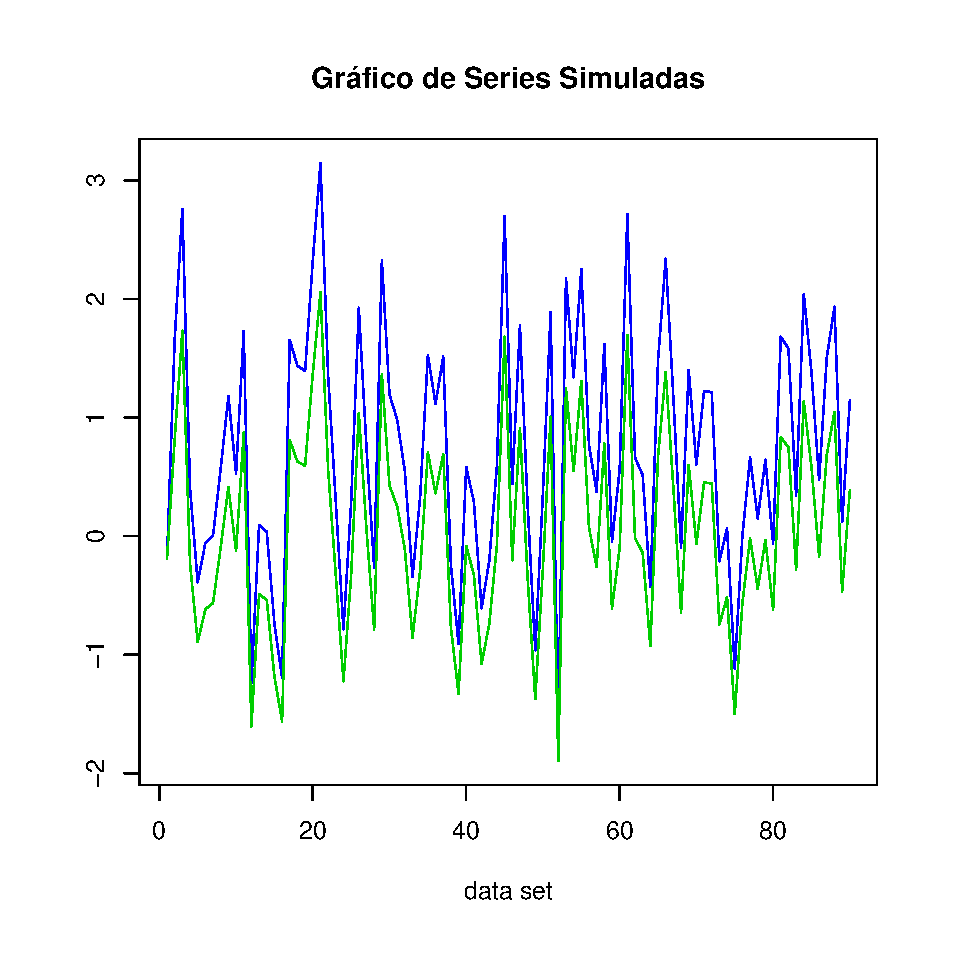
\includegraphics[height=5cm, width=6cm]{rho_1.ps}
  \caption{Valores de $\hat{\rho}_{X_{t},Y_{t}} \approx 1$.}
  \label{caja1}
\end{figure}

Cuando se habla del comportamiento de las series de tiempo, se est\'a en presencia de estructuras din\'amicas que no est\'an fijas, como en el caso de las variables aleatorias, ya que se ha calculado que grado de comovimiento tienen, entonces de acuerdo a su definici\'on un $\widehat{\rho}_{X_{t},Y_{t}}(h=1)$ cercano a 1, significa que las series se mueven juntas en cualquier per\'iodo de tiempo $[t_i,t_{i+1}]$.

\subsection{Anti comovimiento}
Estas series fueron simuladas para que el comovimiento entre las dos series este cercano a $-1$.

En el siguiente gr\'afico se puede apreciar un anti comovimiento, es decir, que sus conjuntos de pares de pendientes son inversamente proporcionales.
\begin{figure}[htp]
\centering
  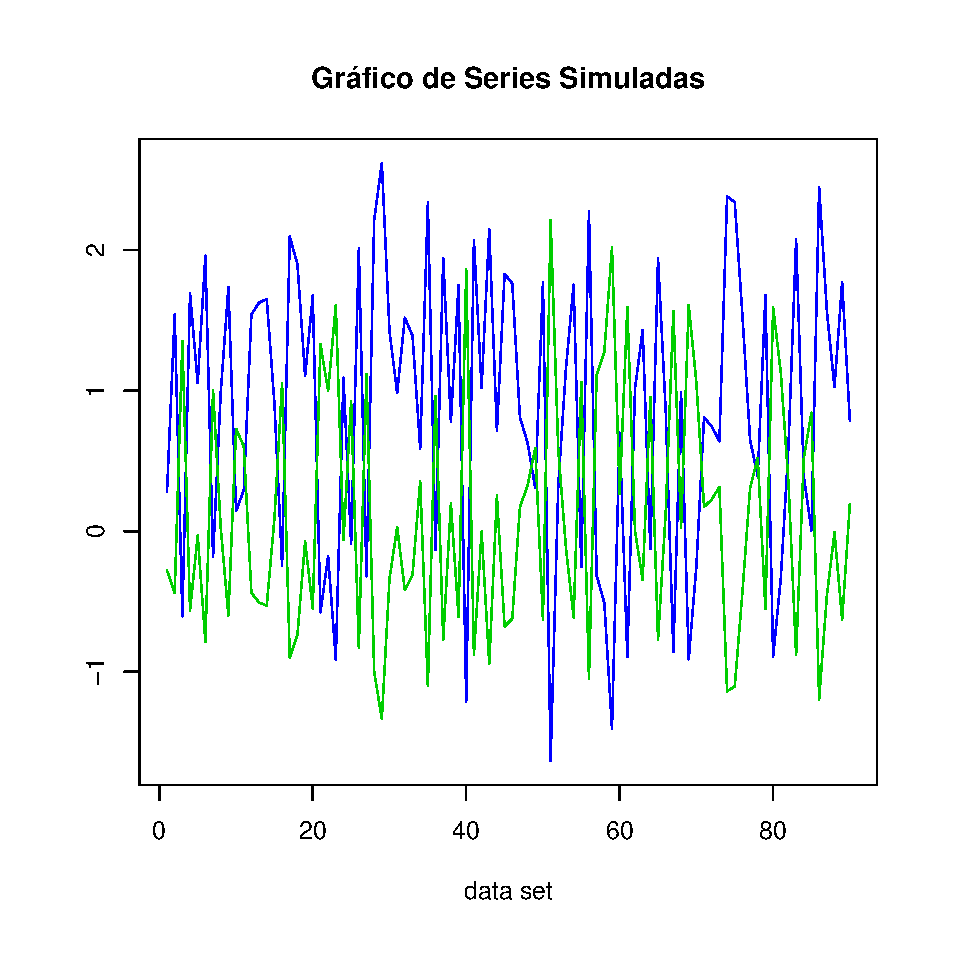
\includegraphics[height=5cm, width=6cm]{rho_-1.ps}
  \caption{Valores de $\hat{\rho}_{X_{t},Y_{t}} \approx -1$.}
  \label{caja2}
\end{figure}
Se puede ver como las series tienen un comportamiento inverso respecto del otro. Si calculamos su grado de comovimiento con el estimador muestral este es $-0.999$. Es decir, estas series comueven de manera inversa en cualquier periodo de tiempo $[t_i,t_{i+1}]$.

\subsection{Comovimiento nulo}
De igual forma, estas series fueron simuladas para que el comovimiento entre las dos series este cercano a $0$.

Finalmente, en este gr\'afico se puede observar que el conjunto de pares de pendientes no tiene nada en com\'un. Es decir, la series en cualquier p\'eriodo de tiempo no comueven. El \'Indice estimado es $0.0001$.

\begin{figure}[htp]
\centering
  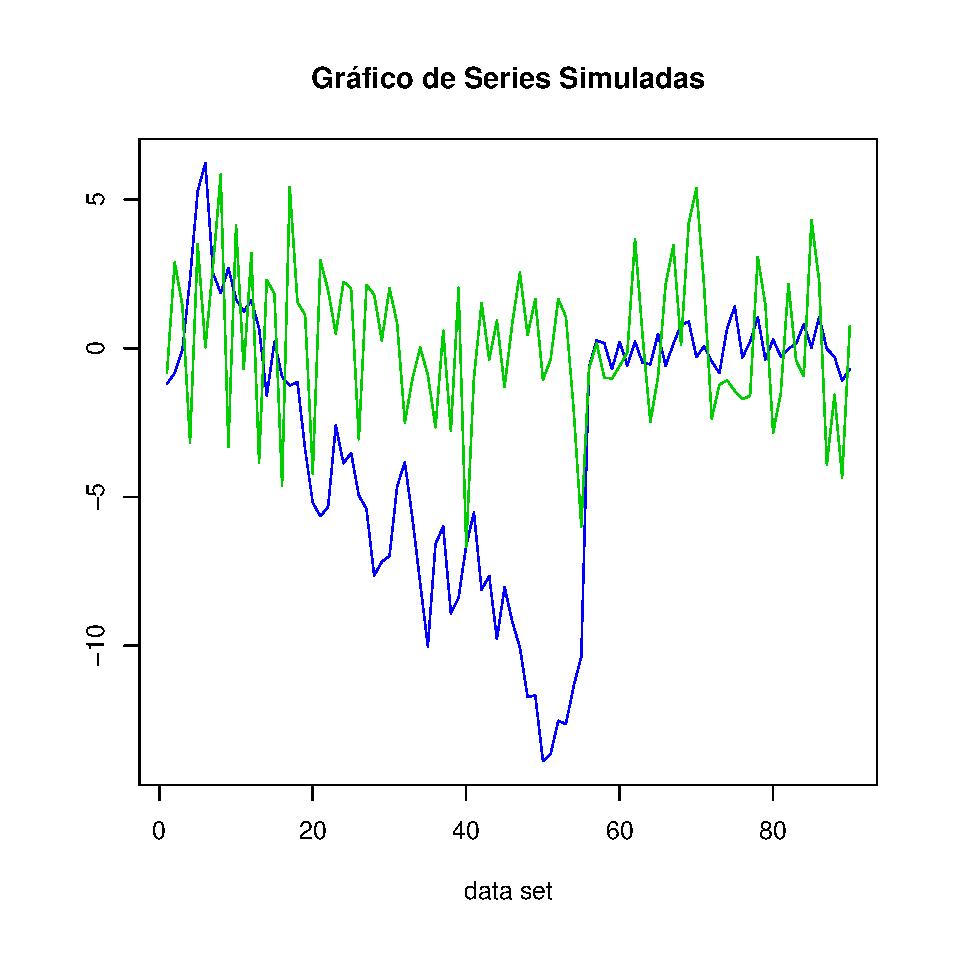
\includegraphics[height=5cm, width=6cm]{rho_0.eps}
   \caption{Valores de $\hat{\rho}_{X_{t},Y_{t}} \approx 0$.}
\label{caja3}
\end{figure}

\section{Propiedades}

Como ya se a dicho, las series de tiempo pueden ser modelados por procesos estoc\'asticos. Esta secci\'on se realizaron los siguientes c\'alculos para dos procesos lineales generales.

Ahora bien, para analizar la similaridad entre dos series de tiempo, se presentar\'an algunos c\'alculos que ser\'an asociados al \'Indice de Comovimiento. La importancia de esta secci\'on es presentar una medida de similaridad expl\'icita, expresada a trav\'es de dos modelos lineales generales. Tambi\'en, se discutir\'a la normalidad asint\'otica del Coeficiente de Codispersi\'on muestral. Entonces, sean dos procesos lineales generales de la forma:

\begin{eqnarray}
X_{t}&=&\sum_{j=0}^{\infty}\phi_{j}\epsilon_{1}(t-j),\\
Y_{t}&=&\sum_{k=0}^{\infty}\theta_{k}\epsilon_{2}(t-k),
\end{eqnarray}

tal que $\sum_{j=0}^{\infty}\phi_{j}< \infty$, $\sum_{k=0}^{\infty}\theta_{k} < \infty$ y $\epsilon_{1}$ y $\epsilon_{2}$ son ruidos blancos con media 0 y varianza $\sigma^{2}$ y $\tau^{2}$ respectivamente. Adem\'as, consideremos la estructura de covarianza para los errores dada por

\begin{eqnarray}
\mathbb Cov(\epsilon_{1}(t),\epsilon_{2}(s)) = \left\{
\begin{array}{cl}
\rho\tau\sigma&\mbox{si } t=s,\\
0&\mbox{en otro caso}.
\end{array}\right.
\end{eqnarray}

Hay varios procesos que satisfacen la forma lineal general, por
ejemplo para procesos autoregresivos de orden 1 y procesos de
media m\'ovil de orden 1. Sin embargo, para procesos ARMA de orden
superior no hay una forma expl\'icita (an\'alitica para $\rho_{X_{t},Y_{t}}(h)$).\\
Ahora se desarrollara los siguientes c\'alculos. Sea:
\begin{eqnarray*}
\mathbb E[X_{t+h}-X_{t}][Y_{t+h}-Y_{t}]&=&\mathbb E[X_{t+h}Y_{t+h}]-\mathbb E[X_{t+h}Y_{t}]-\mathbb E[X_{t}Y_{t+h}]+\mathbb E[X_{t}Y_{t}],
\end{eqnarray*}
\begin{eqnarray*}
\mathbb E[X_{t+h}Y_{t+h}]&=&\mathbb
E\left[\left(\sum_{j=0}^{\infty}{\phi_{j}\epsilon_{1}(t+h-j)}\right)\left(\sum_{k=0}^{\infty}{\theta_{k}\epsilon_{2}(t+h-k)}\right)\right],\\
&=&\sum_{j=0}^{\infty}{\sum_{k=0}^{\infty}{\phi_{j}\theta_{k}}\mathbb
E[\epsilon_{1}(t+h-j)\epsilon_{2}(t+h-k)]},\\
\end{eqnarray*}

Si $t+h-j=t+h-k$, entonces $j=k$. Por lo tanto

\begin{eqnarray*}
\mathbb E[X_{t+h}Y_{t+h}]&=&\sum_{j=0}^{\infty}{\phi_{j}\theta_{j}\rho\tau\sigma}.\\
\mathbb E[X_{t+h}Y_{t}]&=&\mathbb
E\left[\left(\sum_{j=0}^{\infty}{\phi_{j}\epsilon_{1}(t+h-j)}\right)\left(\sum_{k=0}^{\infty}{\theta_{k}\epsilon_{2}(t-k)}\right)\right]\\
&=&\sum_{j=0}^{\infty}{\sum_{k=0}^{\infty}{\phi_{j}\theta_{k}}\mathbb
E[\epsilon_{1}(t+h-j)\epsilon_{2}(t-k)]}
\end{eqnarray*}

Si $t+h-j=t-k$, entonces $j=k+h$. Luego

\begin{eqnarray*}
\mathbb E[X_{t+h}Y_{t}]&=&\sum_{j=0}^{\infty}{\phi_{k+h}\theta_{k}\rho\tau\sigma.}\\
\mbox{Adem\'as,   } \mathbb E[X_{t+h}Y_{t}]&=&\sum_{j=0}^{\infty}{\phi_{j+h}\theta_{j}\rho\tau\sigma.}\mbox{    Similarmente,  }\\
\mathbb E[X_{t}Y_{t+h}]&=&\mathbb
E\left[\left(\sum_{j=0}^{\infty}{\phi_{j}\epsilon_{1}(t-j)}\right)\left(\sum_{k=0}^{\infty}{\theta_{k}\epsilon_{2}(t+h-k)}\right)\right]\\
\end{eqnarray*}
\begin{eqnarray*}
&=&\sum_{j=0}^{\infty}{\sum_{k=0}^{\infty}{\phi_{j}\theta_{k}}\mathbb
E[\epsilon_{1}(t-j)\epsilon_{2}(t+h-k)]}\\
\mbox{Si $t-j=t+h-k$, entonces $k=j+h$}\\
\mathbb E[X_{t}Y_{t+h}]&=&\sum_{j=0}^{\infty}{\phi_{j}\theta_{j+h}\rho\tau\sigma.}\mbox{  Finalmente,  }\\
\mathbb E[X_{t}Y_{t}]&=&\mathbb
E\left[\left(\sum_{j=0}^{\infty}{\phi_{j}\epsilon_{1}(t-j)}\right)\left(\sum_{k=0}^{\infty}{\theta_{k}\epsilon_{2}(t-k)}\right)\right]\\
&=&\sum_{j=0}^{\infty}{\sum_{k=0}^{\infty}{\phi_{j}\theta_{k}}\mathbb
E[\epsilon_{1}(t-j)\epsilon_{2}(t-k)]}\\
\mbox{Si $t-j=t-k$, entonces $k=j$. Por lo tanto, }\\
\mathbb E[X_{t}Y_{t}]&=&\sum_{j=0}^{\infty}{\phi_{j}\theta_{j}\rho\tau\sigma}\\
\mbox{Note que $\mathbb E[X_{t+h}Y_{t+h}]=\mathbb E[X_{t}Y_{t}]$}
\end{eqnarray*}

Para el c\'alculo del denominador del coeficiente se tiene que

\begin{eqnarray*}
\mathbb E[X_{t+h}-X_{t}]^{2}&=&\mathbb Var[X_{t+h}-X_{t}]=\mathbb Var[X_{t+h}]+\mathbb Var[X_{t}]-2\mathbb Cov[X_{t+h}X_{t}].\\
\mathbb Var[X_{t+h}]&=&\mathbb Var\left[\sum_{j=0}^{\infty}\phi_{j}\epsilon_{1}(t+h-j)\right]=\sum_{j=0}^{\infty}\phi_{j}^{2}\mathbb Var[\epsilon_{1}(t+h-j)]=\sum_{j=0}^{\infty}\phi_{j}^{2}\sigma^{2}.\\
\mathbb Var[X_{t}]&=&\mathbb Var\left[\sum_{j=0}^{\infty}\phi_{j}\epsilon_{1}(t-j)\right]=\sum_{j=0}^{\infty}\phi_{j}^{2}\mathbb E[\epsilon_{1}(t-j)]=\sum_{j=0}^{\infty}\phi_{j}^{2}\sigma^{2}.\\
\mathbb Cov[X_{t+h}X_{t}]&=&\mathbb E[X_{t+h}X_{t}]-\mathbb E[X_{t+h}]\mathbb E[X_{t}]=\mathbb E[X_{t+h}X_{t}]\\
\mathbb E[X_{t+h}X_{t}]&=&\mathbb E\left[\left(\sum_{j=0}^{\infty}{\phi_{j}\epsilon_{1}(t+h-j)}\right)\left(\sum_{k=0}^{\infty}{\phi_{k}\epsilon_{1}(t-k)}\right)\right]\\
&=&\sum_{j=0}^{\infty}{\sum_{k=0}^{\infty}{\phi_{j}\phi_{k}}\mathbb
E[\epsilon_{1}(t+h-j)\epsilon_{1}(t-k)]}
\end{eqnarray*}
Si $t+h-j=t-k$, entonces, $k=j+h$
\begin{eqnarray*}
&=&\sum_{j=0}^{\infty}\phi_{j}\phi_{j+h}\sigma^{2}
\end{eqnarray*}
Similarmente, se tiene:
\begin{eqnarray*}
\mathbb E[Y_{t+h}-Y_{t}]^{2}&=&\mathbb Var[Y_{t+h}-Y_{t}]=\mathbb Var[Y_{t+h}]+\mathbb Var[Y_{t}]-2\mathbb
Cov[Y_{t+h}Y_{t}]\\
\mathbb Var[Y_{t+h}]&=&\mathbb Var\left[\sum_{k=0}^{\infty}\theta_{k}\epsilon_{2}(t+h-k)\right]=\sum_{k=0}^{\infty}\theta_{k}^{2}\mathbb Var[\epsilon_{2}(t+h-k)]=\sum_{k=0}^{\infty}\theta_{k}^{2}\tau^{2}.\\
\end{eqnarray*}
\begin{eqnarray*}
\mathbb Var[Y_{t}]&=&\mathbb Var\left[\sum_{k=0}^{\infty}\theta_{k}\epsilon_{2}(t-k)\right]=\sum_{j=0}^{\infty}\theta_{k}^{2}\mathbb Var[\epsilon_{2}(t-k)]=\sum_{k=0}^{\infty}\theta_{k}^{2}\tau^{2}.\\
\mathbb Cov[Y_{t+h}Y_{t}]&=&\mathbb E[Y_{t+h}Y_{t}]-\mathbb E[Y_{t+h}]\mathbb E[Y_{t}]=\mathbb E[Y_{t+h}Y_{t}]\\
\mathbb E[Y_{t+h}Y_{t}]&=&\mathbb E\left[\left(\sum_{j=0}^{\infty}{\theta_{j}\epsilon_{2}(t+h-j)}\right)\left(\sum_{k=0}^{\infty}{\theta_{k}\epsilon_{2}(t-k)}\right)\right]\\
&=&\sum_{j=0}^{\infty}{\sum_{k=0}^{\infty}{\theta_{j}\theta_{k}}\mathbb
E[\epsilon_{1}(t+h-j)\epsilon_{1}(t-k)]}
\end{eqnarray*}
Si $t+h-j=t-k$, entonces, $k=j+h$
\begin{eqnarray*}
\mathbb E[Y_{t+h}Y_{t}]&=&\sum_{j=0}^{\infty}\theta_{k}\theta_{k+h}\tau^{2}
\end{eqnarray*}

Ahora si juntamos los t\'erminos y factorizamos nos queda.
\begin{eqnarray*}
\rho_{X_t,Y_t}(h)&=&\rho\cdot\frac{\sum_{j=0}^{\infty}(2\phi_{j}\theta_{j}-\phi_{j+h}\theta_{j}-\phi_{j}\theta_{j+h})}{2\sqrt{\sum_{j=0}^{\infty}(\phi_{j}^{2}-\phi_{j}\phi_{j+h})\sum_{j=0}^{\infty}(\theta_{j}^{2}-\theta_{j}\theta_{j+h})}}.
\end{eqnarray*}

Como caso particular:\\
Cuando ${X_{t}}$ $\sim$ AR(1) y ${Y_{t}}$ $\sim$ AR(1), los param\'etros $\phi$ y $\theta$ satisfacen $\phi_{j}=\phi^{j}$ ,$|\phi|<1$ y $\theta_{j}=\theta^{j}$, $|\theta|<1$,$|\theta\phi|<1$

Usando las siguientes identidades.
\begin{eqnarray*}
\sum_{k=0}^{\infty}{\theta^{k}\phi^{k}}=\sum_{k=0}^{\infty}{(\theta\phi)^{k}}&=&\frac{1}{1-\theta\phi},\\
\sum_{k=0}^{\infty}{\theta^{k}\phi^{k+h}}=\phi^{h}\sum_{k=0}^{\infty}{(\theta\phi)^{k}}&=&\frac{\phi^{h}}{1-\theta\phi},\\
\sum_{k=0}^{\infty}{\theta^{k}\phi^{k+h}}=\phi^{h}\sum_{k=0}^{\infty}{(\theta\phi)^{k}}&=&\frac{\phi^{h}}{1-\theta\phi},\\
\sum_{k=0}^{\infty}{\phi^{2k}}&=&\frac{1}{1-\phi^{2}},\\
\sum_{k=0}^{\infty}{\theta^{2k}}&=&\frac{1}{1-\theta^{2}},\\
\sum_{k=0}^{\infty}{\phi^{k}\phi^{k+h}}=\phi^{h}\sum_{k=0}^{\infty}{(\phi)^{2k}}&=&\frac{\phi^{h}}{1-\phi^{2}},\\
\sum_{k=0}^{\infty}{\theta^{k}\theta^{k+h}}=\phi^{h}\sum_{k=0}^{\infty}{(\theta)^{2k}}&=&\frac{\phi^{h}}{1-\theta^{2}},
\end{eqnarray*}
Se tiene
\begin{eqnarray}
\rho_{X_t,Y_t}(h=1)&=&\rho\cdot\frac{(2-\phi-\theta)\sqrt{(1+\phi)(1+\theta)}}{1-\phi\theta}.
\end{eqnarray}
Desde aqu\'i se puede apreciar una forma expl\'icita del Coeficiente de Codispersi\'on $\rho_{X_t,Y_t}(h=1)$. El Coeficiente de Codispersi\'on es una versi\'on corregida del coeficiente de correlaci\'on cl\'asico. Este resultado fue obtenido por Rukhin y Vallejos (2008). Las propiedades asint\'oticas de  $\widehat{\rho}(h)$ fueron establecidas para el proceso $\mathbb Z_{s}=(\mathbb X_{s},\mathbb Y_{s})^{t}$ admitiendo la siguiente estructura,
\begin{eqnarray}
\mathbb Z_{s+h}-\mathbb Z_{s}=\sum_{l}\mathbb A_{l}\epsilon_{s-l},
\end{eqnarray}
Donde $\mathbb A_{l}=\mathbb A_{h}(l)$ son matrices $2 \times 2$ definida para todo $l$ tal que, $\sum\|\mathbb A(l)\|^{2}<\infty$, donde $\|\cdot\|$ denota cualquier norma matricial y $\epsilon_{t}$ son vectores independientes con media cero y matriz de covarianza $\Sigma$.

\begin{thm}{\rm
  Si el valor observado admite la representaci\'on del proceso $Z_{t}=(X_{t},Y_{t})^{t}$ (1.8.5) con matrices
  $A(k,l)=diag(\alpha_{kl},\beta_{kl})$, la distribuci\'on limite
  de $M[\hat{\rho_{X,Y}(h)-\rho}]$ es normalmente distribu\'ida con media 0 y
  varianza
  \begin{eqnarray}
  \nu^{2}&=&\left(1-\frac{\rho^{2}\sum_{s=0}^{\infty}{(\alpha_{s}\beta_{s})^{2}}}{\sum_{s=0}^{\infty}{\alpha_{s}^{2}}\sum_{s=0}^{\infty}{\beta_{s}^{2}}}\right).
  \end{eqnarray}
}
\end{thm}
Con este resultado, se han realizados trabajos con D\'ocimas de hip\'otesis, intervalos de Confianza y Bandas de confianzas para el Coeficiente de Codispersi\'on (Ver Rukhin y Vallejos, 2008).

La ventaja de encontrar una forma expl\'icita para la varianza del coeficiente facilita los c\'alculos para d\'ocimar y encontrar intervalos de Confianza ya que en caso contrario, habr\'ia que calcular la varianza, a trav\'es, de m\'etodos de re-muestreo.

\section{Limitaciones te\'oricas}

Dentro de las limitaciones te\'oricas se puede mencionar que para modelos con muchos pa\-r\'a\-me\-tros no existe una forma anal\'itica para el coeficiente, en este caso es necesario implementar t\'ecnicas computacionales. Cabe,
mencionar que para series de tiempo no estacionarias el \'indice de codispersi\'on no ha sido estudiado. Cuando una de las series presenta outliers, el coeficiente de codispersi\'on es muy sensible. La definici\'on de una version robusta del coeficiente de Codispersi\'on a\'un es un problema abierto.

\section{M\'etodos no par\'ametricos}

En la literatura existe una medida de asociac\'ion para procesos espaciales. Tj$\phi$stheim (1978), propone una medida de asociaci\'on para variables espaciales, esta medida est\'a basada en los rangos de las observaciones y la localizaci\'on de las coordenadas de los puntos medios. 